\section{Zustandsmaschiene}
\subsection{UML}
\begin{center}
	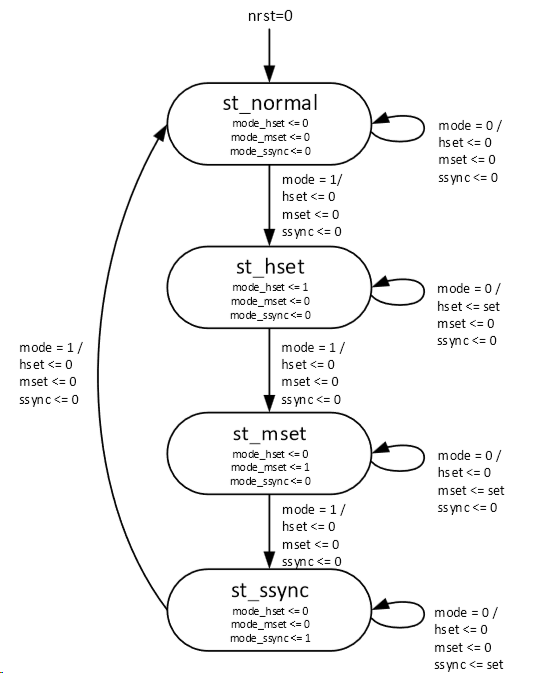
\includegraphics[width=\columnwidth]{Images/zustandsmachine}
\end{center}



\subsection{Sequentielle Systeme - FSM}
Im Gegensatz zu Kombinatorischen Systeme, sind sequentielle Systeme Zustandsbehaftet. Vergangene Verhalten und Eingänge bestimmen momentane Ausgabe, diese sind immer mit einem Takt synchronisiert.
\begin{lstlisting}
	library ieee;
	
	entity fsm is
	port(
	clk : in bit;
	rst : in bit;
	inp : in bit_vector(m-1 downto 0);
	oup : out bit_vector(n-1 downto 0);
	);
	end;
	
	architecture behavioral of fsm is
	-- type
	type state_type is (st_reset, st1, st2, ...);
	-- register
	signal present_state, next_state: state_type;
	begin
	-- siehe spezifische FSM
	end;
\end{lstlisting}
Im folgenden sind 3-Prozesse Strukturen definiert, für 2-Prozesse können Prozess F und G in einem abgehandelt werden, dafür muss aber die sensitivitäts-Liste angepasst werden.


\subsubsection{Mealy Struktur}
Wert der Ausgänge ist von Eingängen und Zuständen Abhängig. Eingänge gehen asynchron durch. Kann zu \underline{Timing Problemen} führen!

\begin{center}
	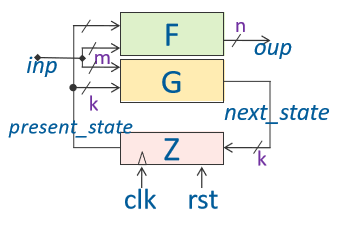
\includegraphics[width=0.4\columnwidth]{Images/mealy_fsm} 
\end{center}
\begin{lstlisting}
	-- Process F
	output_logic: process(inp, present_state)
	begin
	-- default
	oup <= "00";
	
	if (present_state = st1 and inp = "10") then
	oup <= "10";
	-- alle States inkl else
	end if;
	end process;
	
	-- Process G
	next_state_logic: process(inp, present_state)
	begin
	-- default
	next_state <= st_reset;
	
	case present_state is -- folgezustand
	when st1 =>
	if (inp = "10") then
	next_state <= st2;
	end if;
	when ..
	when others => null
	end case;
	end process;
	
	-- Process Z
	state_register: process (clk)
	begin
	if (rising_edge(clk)) then
	if (rst = '1') then
	present_state <= st_reset;
	else 
	present_state <= next_state;
	end if
	end process;
\end{lstlisting}


\subsubsection{Moore Struktur}
Wert der Ausgänge ist nur vom aktuellen Zustand des Systems abhängig.

\begin{center}
	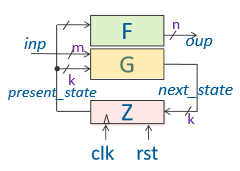
\includegraphics[width=0.4\columnwidth]{Images/moor_fsm}
\end{center}
\begin{lstlisting}
	-- Process F
	output_logic: process(present_state)
	begin
	-- default
	oup <= "00";
	
	if (present_state = st1) then
	oup <= "10";
	-- alle States inkl else
	end if;
	end process;
	
	-- Process G
	next_state_logic: process(inp, present_state)
	begin
	-- ..
	end process;
	
	-- Process Z
	state_register: process (clk)
	begin
	-- ..
	end process;
\end{lstlisting}

\subsubsection{Medwedjew Struktur}
Spezialfall des Moore-Systems: Ausgänge entsprechen dem Zustandsvektor. zB für Zähler.

\begin{center}
	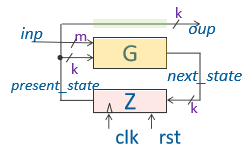
\includegraphics[width=0.4\columnwidth]{Images/med_fsm}
\end{center}
\begin{lstlisting}
	-- Process G
	next_state_logic: process(inp, present_state)
	begin
	-- ..
	end process;
	
	-- Process Z
	state_register: process (clk)
	begin
	-- ..
	end process;
	
	oup <= present_state
\end{lstlisting}

